\section{Tainting dependencies}
\label{sect:impl:tainting_deps}
Tainting Dependencies is a method of translating XQuery queries to
relational algebra. The semantics of this method is described in detail
throughout Chapter \ref{sect:translation}. This section
describes an implementation of a subset of the rules in this method -- an
implementation which is capable of translating simple FLWOR expressions,
sequences, and variables.

\subsection{Tainting}
\label{sect:impl:taint:taint}
The concept of tainting one expression with the iterator dependencies of another is described in section
\ref{sect:trans:TD:tainting} on page \pageref{sect:trans:TD:tainting}. A method
\texttt{taint()} is introduced to cover the semantics of this concept.
Residing in the \textit{XQuery2MQL visitor} class it is reachable from all nodes of the tree. The method is implemented like this:

\begin{Verbatim}
protected TraverseReturn taint(TraverseReturn tr, VarRefSet varRefs) {
        
    TraverseReturn result = new TraverseReturn();
        
    VarRefSet taintBy = (VarRefSet)varRefs.clone();
    taintBy.removeAll(tr.getVarRefs());
        
    Operator expr = tr.getOperatorTree();
    Project project;
    for (VarRef varRef : taintBy) {
        project = new Project(varRef.getName() + "numb",
                      Scope.get(varRef.getName()).getOperatorTree());
        expr = new Cross(project, expr);
    }

    tr.getVarRefs().addAll(taintBy); \\ Add gained dependencies
    result.setVarRefs(tr.getVarRefs());
    result.setOperatorTree(expr);
    result.setSingleton(tr.isSingleton());
        
    return result;
}
\end{Verbatim}

\subsection{FLWOR expressions}
The translation process for FLWOR expressions was outlined in section
\ref{sect:trans:TD:simpleFLWOR}. Consider inference rule
\ref{rule:trans:TD:forbind} on page \pageref{rule:trans:TD:forbind}. This
inference rule states how to translate and bind an iterator variable in a
\texttt{for}-clause in a FLWOR expressions. Furthermore, consider the abstract
syntax tree example in Figure \ref{fig:impl:td:flwor2}. First a
\texttt{for}-clause is visited, and the  child is flagged as a FLWOR tuplet
definition.
% \begin{Verbatim}
% public TraverseReturn visitAST_FORCLAUSE(XQFTTree tree) {
% 
%     ((XQFTTree)tree.getChild(0)).setFlworTupleDef(true);
%     acceptThis(tree.getChild(0));
%     return null;
% }
% \end{Verbatim}

\begin{figure}[!htp]
\begin{center}
  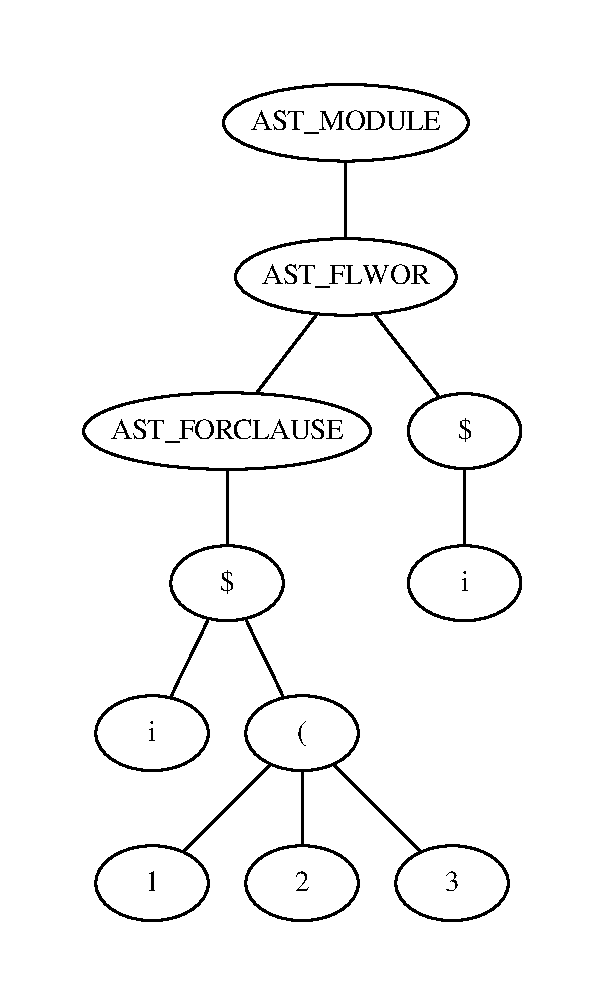
\includegraphics[scale=0.4]{img/graphs/flwor2}
  \caption{FLWOR syntax tree example}
  \label{fig:impl:td:flwor2}
\end{center}
\end{figure} 

Next a dollar sign is visited (which carries the meaning of a variable in the
abstract syntax tree). If the child count is more than one, it is an
assignment. Note that the \texttt{isIterationVar} flag is \textit{true} if
this assignment is a tuple definition as flagged earlier. Then, if this is an
assignment and a tuple definition, the right-hand side of the assignment is
translated, and the symbol is entered into a symbol table. The
creation of the project operator is required by inference rule
\ref{rule:trans:TD:forbind}:

\begin{Verbatim}     
    // Visit children on the right side of the assignment
    TraverseReturn tr = acceptThis(tree.getChild(1));
        
    // Augment with -numb attribute
    Project project = new Project(varName + "numb, index=1, value", 
       tr.getOperatorTree());

    // Assign metadata
    tr.setOperatorTree(project);
    tr.setSingleton(true);
     
    // Enter into symbol table
    SymTabEntry tmp = Scope.set(tree.getChild(0).getText(), 
                          tr, isIterationVar);
     
    if (tree.isFlworTupleDef()) {
       Scope.setCurrentIterVar(new VarRef(tmp.getName()));
    }
\end{Verbatim}



Following the translation of the \texttt{for}-clause, the
\texttt{return}-clause and its subexpressions are translated. When the visitor returns to the AST\_FLWOR node, as there is no \texttt{where} or \texttt{order
by}-clauses iterator ordering (Section \ref{sect:trans:TD:flwor:itOrd}, page \pageref{sect:trans:TD:flwor:itOrd})
is applied:

\begin{Verbatim}
    ...
    // Taint if needed
    returnClause = this.taint(returnClause, Scope.getCurrentIterVar());

    // Remove current iterator from dependencies
    VarRefSet newVarRefs 
    	= (VarRefSet)returnClause.getVarRefs().clone();         
    newVarRefs.remove(Scope.getCurrentIterVar());

    // Sort and partition fields
    String[] sortBy = {Scope.getCurrentIterVar().getName() 
    		          + "numb", "index"};
    String[] partitionBy 
    	= new String[returnClause.getVarRefs().size() - 1];

    int i = 0;
    for (VarRef ref : prevVarRefs) {
        partitionBy[i] = ref.getName();
        i++;
    }

    // Construct MQL
    Numberate numberate = new Numberate("index", 
                                        sortBy, 
                                        partitionBy, 
                                        returnClause.getOperatorTree());

    // Construct result
    TraverseReturn result = new TraverseReturn();
    result.setSingleton(false);
    result.setVarRefs(newVarRefs);
    result.setOperatorTree(numberate);

    Scope.pop();
    return result;
\end{Verbatim}

\subsection{Sequences}
\label{sect:impl:td:seq}
The translation process for sequence construction is described in section
\ref{sect:trans:TD:seqBuild}. First, the iterator dependencies of the expression is calculated. This is used to
taint all the subexpressions:

\begin{Verbatim}
    boolean allSingletons = true;    

    // Collect all iterator dependencies
    VarRefSet allVarRefs = new VarRefSet();
    for (TraverseReturn childResult : childResults) {
        allVarRefs.addAll(childResult.getVarRefs());
        if(!childResult.isSingleton())
            allSingletons = false;
    }

    Union union = new Union();

    for (TraverseReturn childResult : childResults) {
        if(allSingletons)
            projectString = "index = " + c + ", value";
        else
            projectString = "sprIdx = " + c + ", index, value";

        union.addOperator(new Project(projectString, 
                this.taint(childResult, allVarRefs).getOperatorTree()))
        c++;    
    }
    
    if(!allSingletons)
        ...
\end{Verbatim}

The tainted expressions are added to an \textsf{union} operator. But first they will have to be inserted into a
\textsf{project} operator, with parameters depending on they are all singleton sequences or not. If they are, the
union is wrapped in a \texttt{TraverseReturn}, completing the translation of the sequence constructor. If they are
not, a \textsf{numberate} operator is needed.

Note that the parantheses in sequence expressions are not required, and
according to specification, sequence expressions are recognised by the comma
symbols and not parantheses. However, the XQFT Parser rewrites sequence
expressions into including a paranthesis as start token for sequence subtrees
within the AST.

\subsection{If-then-else}
The translation process for conditional expressions is explained in section
\ref{sect:trans:TD:ifThenElse}. In particular, rule
\ref{rule:trans:TD:conditional} describes this translation. 
% \begin{Verbatim}
% // if (e1) then e2 else e3
% XQFTTree e1 = (XQFTTree)tree.getChild(0); 
% XQFTTree e2 = (XQFTTree)tree.getChild(1);
% XQFTTree e3 = (XQFTTree)tree.getChild(2);
%         
% // Visit the expressions
% TraverseReturn r_e1 = acceptThis(e1);
% TraverseReturn r_e2 = acceptThis(e2);
% TraverseReturn r_e3 = acceptThis(e3);
% \end{Verbatim}

First the child expressions are visited, and the variables \texttt{e1},
\texttt{e2}, and \texttt{e3} correspond to the expressions $e_1$, $e_2$, and
$e_3$ in Rule \ref{rule:trans:TD:conditional},  while \texttt{r\_e1},
\texttt{r\_e3}, and \texttt{r\_e3} correspond to \textbf{r}($e_1$),
\textbf{r}($e_2$), and \textbf{r}($e_3$).

Continuing, sets of iterator dependencies are obtained:
         
\begin{Verbatim}
// VarRefs: e2 union e3
VarRefSet v_e2_u_e3 = (VarRefSet)r_e2.getVarRefs().clone();
v_e2_u_e3.addAll(r_e3.getVarRefs());

// VarRefs: (e2 union e3) intersect e1
VarRefSet v_e2_u_e3_i_e1 = (VarRefSet)v_e2_u_e3.clone();
v_e2_u_e3_i_e1.retainAll(r_e1.getVarRefs());

// VarRefs: e1 union e2 union e3
VarRefSet v_e1_u_e2_u_e3 = (VarRefSet)r_e1.getVarRefs().clone();
v_e1_u_e2_u_e3.addAll(r_e2.getVarRefs());
v_e1_u_e2_u_e3.addAll(r_e3.getVarRefs());
\end{Verbatim}

The variable \texttt{v\_e2\_u\_e3} corresponds to $e_2 \cup e_3$, \texttt{v\_e2\_u\_e3\_i\_e1} corresponds to
$(e_2 \cup e_3) \cap e_1$, and \texttt{v\_e1\_u\_e2\_u\_e3} corresponds to $e_2 \cup e_3 \cup
e_1$.

This result is used to create the to \textsf{project()} operators and union
them together:

\begin{Verbatim}
// Alternatives
Project alt1 = new Project("index, alt=1, " + v_e2_u_e3.toStringList() + ", value", 
                      this.taint(r_e2, r_e3.getVarRefs()).getOperatorTree()); 

Project alt2 = new Project("index, alt=2, " + v_e2_u_e3.toStringList() + ", value", 
                      this.taint(r_e3, r_e2.getVarRefs()).getOperatorTree()); 

// Union
Union union = new Union(alt1, alt2);
\end{Verbatim}

The translation is finalised by using this result to construct a join and apply
the \textsf{select()} operator:

\begin{Verbatim}
// HHjoin
HHJoin hhjoin = new HHJoin("[" + v_e2_u_e3_n_e1.toStringList() + "]," +
                           "[" + v_e2_u_e3_n_e1.toStringList() + "]," + 
                           "[index = l.index, " + v_e1_u_e2_u_e3.toStringList() +
                           ", lvalue = l.value, rvalue = r.value]", 
                             union, r_e1.getOperatorTree());

// Select
Select select = new Select("ifthenelse(xqBoolean(rvalue), 
                    eq(alt,1), eq(alt,2))", hhjoin);

// Project
Project project = new Project("index, " + 
                  v_e1_u_e2_u_e3.toStringList() +
                  ", value = lvalue" , select);
\end{Verbatim}
